\chapter{Máquinas de vectores de soporte}\label{Chapter8} 
% chktex-file 8
% chktex-file 12
% chktex-file 13
% chktex-file 44

Se ha demostrado que las SVMs funcionan bien en una variedad de entornos y a menudo se consideran uno de los mejores clasificadores ``listos para usar''. \\

La máquina de vectores de soporte es una generalización de un clasificador simple e intuitivo llamado clasificador de máximo margen, Aunque es elegante y simple,  este clasificador no se puede aplicar a la mayoría de los conjuntos de datos, ya que requiere que las clases sean separables por un límite lineal. El clasificador de vectores de soporte es una extensión del clasificador de máximo margen que se puede aplicar en una gama más amplia de casos. Finalmente, la máquina de vectores de soporte es una extensión adicional del clasificador de vectores de soporte para acomodar límites de clase no lineales. Las máquinas de vectores de soporte están destinadas al entorno de clasificación binaria en el que hay dos clases. 

\section{Clasificador de máximo margen}

\subsection{Hiperplano}

En un espacio p-dimensional, un hiperplano es un subespacio afín plano de dimensión $p - 1$. Por ejemplo, en dos dimensiones, un hiperplano es un subespacio plano unidimensional, en otras palabras, una línea. En tres dimensiones, un hiperplano es un subespacio plano bidimensional, es decir, un plano. La definición matemática de un hiperplano es bastante simple. En dos dimensiones, un hiperplano se define por la ecuación
\begin{equation}
\beta_0 + \beta_1 X_1 + \beta_2 X_2 = 0
\label{eq:9.1}
\end{equation}

para los parámetros $\beta_0$, $\beta_1$ y $\beta_2$. Cuando decimos que esta ecuación define el hiperplano, queremos decir que cualquier $X = (X_1, X_2)^T$ para el cual se cumple esta ecuación es un punto en el hiperplano. La ecuación anterior puede extenderse fácilmente al entorno p-dimensional:
\begin{equation}
\beta_0 + \beta_1 X_1 + \beta_2 X_2 + \ldots + \beta_p X_p = 0
\label{eq:9.2}
\end{equation}

define un hiperplano p-dimensional, nuevamente en el sentido de que si un punto $X = (X_1, X_2, \ldots, X_p)^T$ en el espacio p-dimensional (es decir, un vector de longitud $p$) satisface esta ecuación, entonces $X$ se encuentra en el hiperplano. \\

\noindent Ahora, supongamos que $X$ no satisface la ecuación (\ref{eq:9.2}); más bien,
\begin{equation}
\beta_0 + \beta_1 X_1 + \beta_2 X_2 + \ldots + \beta_p X_p > 0.
\end{equation}

\noindent Entonces esto nos dice que $X$ se encuentra a un lado del hiperplano. Por otro lado, si
\begin{equation}
\beta_0 + \beta_1 X_1 + \beta_2 X_2 + \ldots + \beta_p X_p < 0,
\end{equation}

entonces $X$ se encuentra al otro lado del hiperplano. Así que podemos pensar en el hiperplano como una divisón del hiperespacio en dos mitades. Uno puede determinar fácilmente en qué lado del hiperplano Un hiperplano en el espacio bidimensional se muestra en la figura \ref{fig:9.1}.

\begin{figure}[h]
\centering
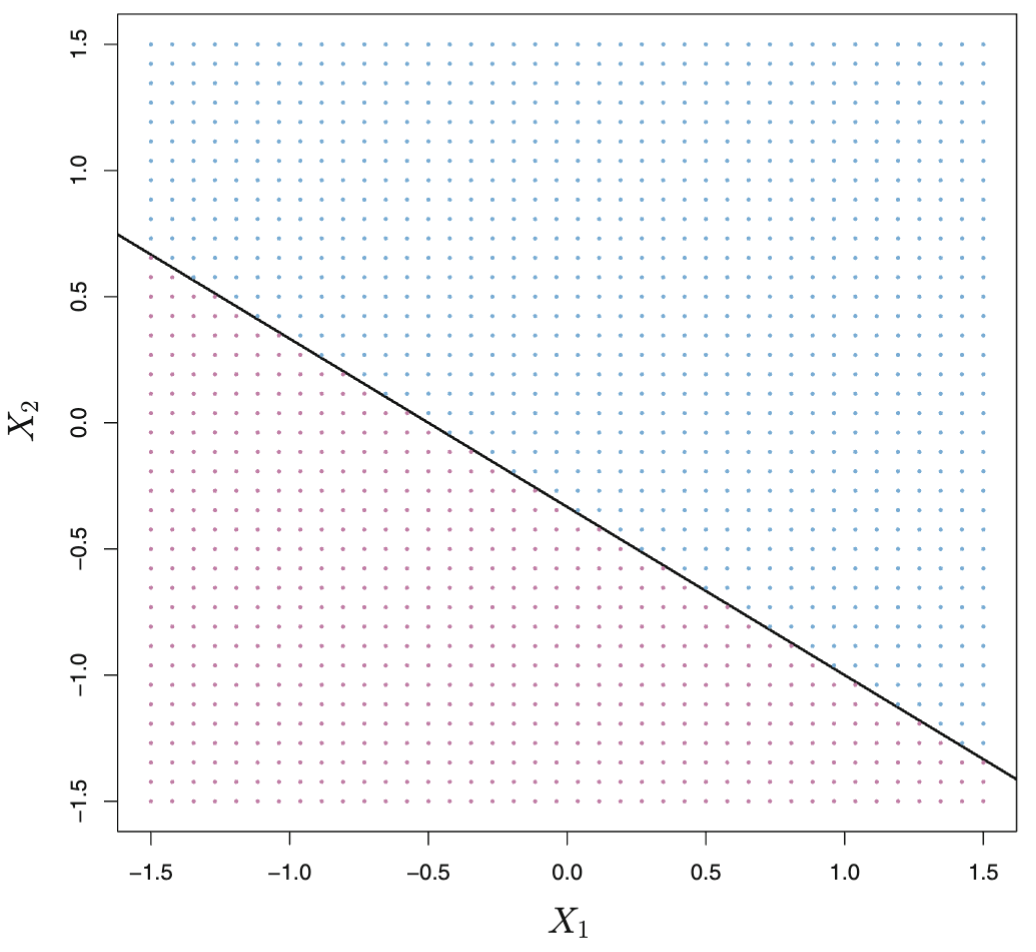
\includegraphics[width=0.5\textwidth]{fotos/52.png}
\caption{Hiperplano $1 + 2X_1 + 3X_2 = 0$. La región azul consiste en los puntos tales que $1 + 2X_1 + 3X_2 > 0$, mientras que la región roja consiste en los puntos tales que $1 + 2X_1 + 3X_2 < 0$.}
\label{fig:9.1}
\end{figure}

\subsection{Clasificación usando un hiperplano separador}

Ahora supongamos que tenemos una matriz de datos $n \times p$ $\mathbf{X}$ consistente en $n$ observaciones de entrenamiento en un espacio p-dimensional,
\begin{equation}
x_1 =
\begin{pmatrix}
x_{11} \\
\vdots \\
x_{1p}
\end{pmatrix}, \ldots, x_n =
\begin{pmatrix}
x_{n1} \\
\vdots \\
x_{np}
\end{pmatrix},
\end{equation}
y que estas observaciones caen en dos clases, es decir, $y_1, \ldots, y_n \in \{-1, 1\}$ donde $-1$ representa una clase y $1$ la otra clase. También tenemos una observación de prueba, un vector p-dimensional de características observadas $x^* = (x^*_1, \ldots, x^*_p)^T$. Nuestro objetivo es desarrollar un clasificador basado en los datos de entrenamiento que clasifique correctamente la observación de prueba utilizando sus mediciones de características. Lo haremos con un nuevo enfoque basado en el concepto de un hiperplano separador. \\

\begin{figure}[h]
\centering
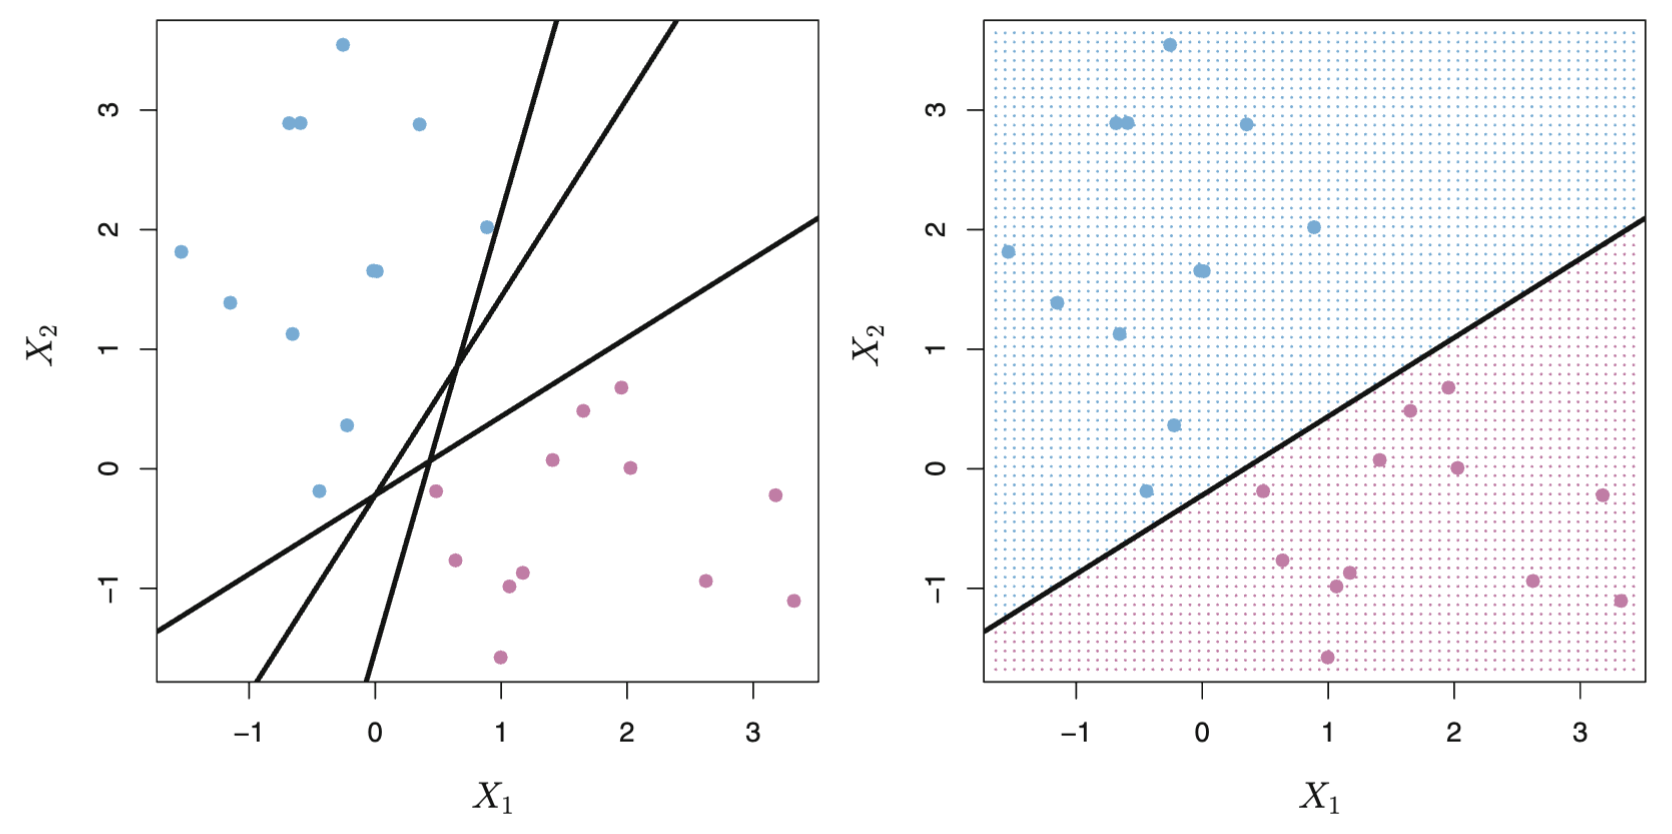
\includegraphics[width=\textwidth]{fotos/53.png}
\caption{Izquierda: hay dos clases de observaciones (en distintos colores), cada una con medidas en dos variables. Se muestran tres posibles hiperplanos separadores en negro. Derecha: se muestra un ejemplo de hiperplano separador, los ejemplos que caigan en la zona azul serán clasificados como esa clase, mientras que los que caigan en la región morada, serán clasificados como de esa clase.}
\label{fig:9.2}
\end{figure}

Supongamos que es posible construir un hiperplano que separe perfectamente las observaciones de entrenamiento según sus etiquetas de clase. Ejemplos de tres de estos hiperplanos separadores se muestran en el panel izquierdo de la figura \ref{fig:9.2}. Podemos etiquetar las observaciones de la clase azul como $y_i = 1$ y las de la clase púrpura como $y_i = -1$. Entonces, un hiperplano separador tiene la propiedad de que
\begin{align}
\beta_0 + \beta_1 x_{i1} + \beta_2 x_{i2} + \ldots + \beta_p x_{ip} > 0 &\text{ si } y_i = 1, \\
\beta_0 + \beta_1 x_{i1} + \beta_2 x_{i2} + \ldots + \beta_p x_{ip} < 0 &\text{ si } y_i = -1.
\end{align}

\noindent De manera equivalente, un hiperplano separador tiene la propiedad de que
\begin{equation}
y_i (\beta_0 + \beta_1 x_{i1} + \beta_2 x_{i2} + \ldots + \beta_p x_{ip}) > 0
\end{equation}

\noindent para todo $i = 1, \ldots, n$. \\

Si existe un hiperplano separador, podemos usarlo para construir un clasificador muy natural: una observación de prueba se asigna a una clase dependiendo de en qué lado del hiperplano se encuentra. El panel derecho de la figura \ref{fig:9.2} muestra un ejemplo de tal clasificador. Es decir, clasificamos la observación de prueba $x^*$ basándonos en el signo de 
\begin{equation}
f(x^*) = \beta_0 + \beta_1 x^*_1 + \beta_2 x^*_2 + \ldots + \beta_p x^*_p
\end{equation}

Si $f(x^*)$ es positivo, entonces asignamos la observación de prueba a la clase 1, y si $f(x^*)$ es negativo, entonces la asignamos a la clase -1. También podemos hacer uso de la magnitud de $f(x^*)$. Si $f(x^*)$ está lejos de cero, esto significa que $x^*$ está lejos del hiperplano, por lo que podemos estar seguros de nuestra asignación de clase para $x^*$. Por otro lado, si $f(x^*)$ está cerca de cero, entonces $x^*$ está cerca del hiperplano, por lo que estamos menos seguros de la asignación de clase para $x^*$. Un clasificador basado en un hiperplano separador conduce, por tanto, a un límite de decisión lineal.

\subsection{Clasificador de máximo margen}

En general, si nuestros datos pueden ser perfectamente separados usando un hiperplano, entonces existirá un número infinito de tales hiperplanos. Para construir un clasificador basado en un hiperplano separador, debemos tener una forma razonable de decidir cuál de los infinitos hiperplanos separadores posibles usar. \\

Una elección natural es el hiperplano de máximo margen (también conocido como el hiperplano separador óptimo), que es el hiperplano separador que está más alejado de las observaciones de entrenamiento. Es decir, podemos calcular la distancia (perpendicular) desde cada observación de entrenamiento hasta un hiperplano separador dado; la menor de estas distancias es la distancia mínima desde las observaciones hasta el hiperplano, y se conoce como el margen. El hiperplano de máximo margen es el hiperplano separador para el cual el margen es mayor, es decir, es el hiperplano que tiene la mayor distancia mínima a las observaciones de entrenamiento. Luego podemos clasificar una observación de prueba según el lado del hiperplano de máximo margen en el que se encuentre. Esto se conoce como el clasificador de máximo margen. Esperamos que un clasificador que tenga un gran margen en los datos de entrenamiento también tenga un gran margen en los datos de prueba, y por lo tanto clasifique correctamente las observaciones de prueba. Aunque el clasificador de máximo margen a menudo tiene éxito, también puede llevar a un sobreajuste cuando $p$ es grande. \\

Si $\beta_0, \beta_1, \ldots, \beta_p$ son los coeficientes del hiperplano de máximo margen, entonces el clasificador de margen máximo clasifica la observación de prueba $x^*$ basándose en el signo de $f(x^*) = \beta_0 + \beta_1 x^*_1 + \beta_2 x^*_2 + \ldots + \beta_p x^*_p$. \\

\begin{figure}[h]
\centering
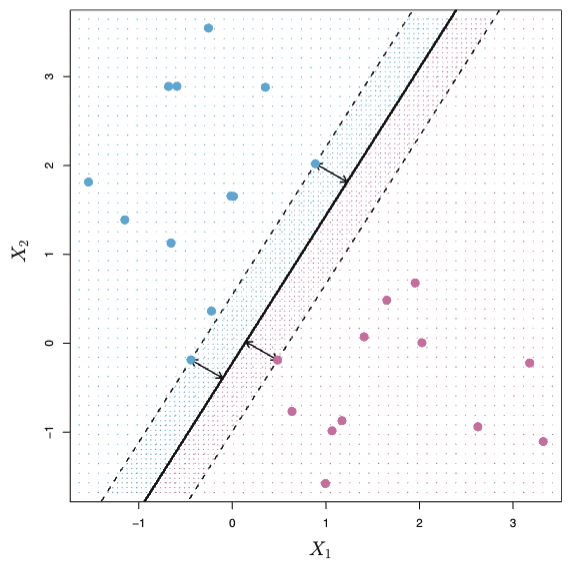
\includegraphics[width=0.5\textwidth]{fotos/54.png}
\caption{Hiperplano de margen máximo.}
\label{fig:9.3}
\end{figure}

La figura \ref{fig:9.3} muestra el hiperplano de margen máximo en el conjunto de datos de la figura \ref{fig:9.2}. Comparando el panel derecho de la figura \ref{fig:9.2} con la figura \ref{fig:9.3}, vemos que el hiperplano de margen máximo mostrado resulta en una mayor distancia mínima entre las observaciones y el hiperplano separador, es decir, un margen mayor. \\

Examinando la figura \ref{fig:9.3}, vemos que tres observaciones de entrenamiento son equidistantes al hiperplano de máximo margen y se encuentran a lo largo de las líneas discontinuas que indican el ancho del margen. Estas tres observaciones se conocen como vectores de soporte, ya que son vectores en el espacio p-dimensional (en esta figura, $p = 2$) y "soportan" el hiperplano de máximo margen en el sentido de que si estos puntos se movieran ligeramente, el hiperplano también se movería. Así, el hiperplano de margen máximo depende directamente de los vectores de soporte, pero no de las otras observaciones: un movimiento de cualquiera de las otras observaciones no afectaría el hiperplano separador, siempre que el movimiento de la observación no cause que cruce el límite establecido por el margen. \\

\subsection{Construcción del clasificador de máximo margen}

Ahora consideramos la tarea de construir el hiperplano de máximo margen basado en un conjunto de $n$ pares de observaciones de entrenamiento $(x_1, y_1) (x_2, y_2), \ldots, (x_n, y_n)$, donde $x_i \in \mathbb{R}^p$ y las etiquetas de clase asociadas $y_i \in \{-1, 1\}$. Brevemente, el hiperplano de margen máximo es la solución al problema de optimización
\begin{align}
\underset{\beta_0, \beta_1, \ldots, \beta_p}{\text{Maximizar }} & M \label{eq:9.9}\\
\text{sujeto a } & \sum_{j = 1}^{p} \beta_j^2 = 1, \label{eq:9.10}\\
& y_i (\beta_0 + \beta_1 x_{i1} + \beta_2 x_{i2} + \ldots + \beta_p x_{ip}) \geq M \quad \forall i = 1, \ldots, n \label{eq:9.11}
\end{align}

\noindent Este problema de optimización es simple. En primer lugar, la restricción 
\begin{equation}
y_i (\beta_0 + \beta_1 x_{i1} + \beta_2 x_{i2} + \ldots + \beta_p x_{ip}) \geq M \quad \forall i = 1, \ldots, n
\end{equation}

garantiza que cada observación estará en el lado correcto del hiperplano, siempre que $M$ sea positivo. De hecho, para que cada observación esté en el lado correcto del hiperplano, simplemente necesitaríamos $y_i (\beta_0 + \beta_1 x_{i1} + \beta_2 x_{i2} + \ldots + \beta_p x_{ip}) > 0$, por lo que la restricción requiere que cada observación esté en el lado correcto del hiperplano, con un cierto margen, siempre que $M$ sea positivo. \\

En segundo lugar, observe que (\ref{eq:9.10}) no es realmente una restricción sobre el hiperplano, ya que si $\beta_0 + \beta_1 x_{i1} + \beta_2 x_{i2} + \ldots + \beta_p x_{ip} = 0$ define un hiperplano, entonces también lo hace $k (\beta_0 + \beta_1 x_{i1} + \beta_2 x_{i2} + \ldots + \beta_p x_{ip}) = 0$ para cualquier $k \neq 0$. Sin embargo, (\ref{eq:9.10}) añade significado a (\ref{eq:9.11}); se puede demostrar que, con esta restricción, la distancia perpendicular desde la $i$-ésima observación al hiperplano está dada por
\begin{equation}
y_i (\beta_0 + \beta_1 x_{i1} + \beta_2 x_{i2} + \ldots + \beta_p x_{ip}).
\end{equation}
Por lo tanto, las restricciones (\ref{eq:9.10}) y (\ref{eq:9.11}) aseguran que cada observación esté en el lado correcto del hiperplano y al menos a una distancia $M$ del hiperplano. Por lo tanto, $M$ representa el margen de nuestro hiperplano, y el problema de optimización elige $\beta_0, \beta_1, \ldots, \beta_p$ para maximizar $M$. 

\subsubsection{Resolución del problema de optimización}

Nuestro conjunto de $n$ obervaciones define un hiperplano que, de forma compacta, podemos escribir como 
\begin{equation}
\{x: f(x) = x^T \beta + \beta_0 = 0\}
\end{equation}

\noindent donde $\beta$ es un vector unitario ($||\beta|| = 1$). Una regla de clasificación inducida por $f(x)$ es 
\begin{equation}
G(x) = \text{sign}(f(x)) = \text{sign}(x^T \beta + \beta_0)
\end{equation}

\begin{figure}[h]
\centering
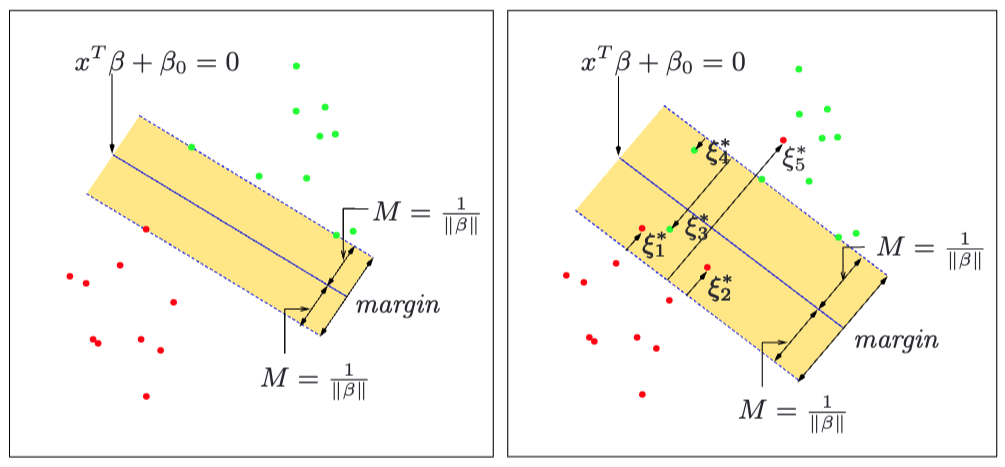
\includegraphics[width=\textwidth]{fotos/56.png}
\caption{Clasificadores de vectores de soporte. El panel izquierdo muestra el caso separable. El límite de decisión es la línea sólida, mientras que las líneas discontinuas delimitan el margen máximo sombreado de ancho $2M = 2/\|\beta\|$. El panel derecho muestra el caso no separable (superposición). Los puntos etiquetados como $\xi^*_j$ están en el lado incorrecto de su margen por una cantidad $\xi^*_j = M \xi_j$; los puntos en el lado correcto tienen $\xi^*_j = 0$, las observaciones que están en el lado incorrecto del margen tienen $\xi_j^* > 0$ y, si $\xi_j^* > 1$, la observación están mal clasificada (en el lado incorrecto del hiperplano). El margen se maximiza sujeto a un presupuesto total $\sum \xi_i \leq \text{constante}$. Por lo tanto, $\sum \xi^*_j$ es la distancia total de los puntos en el lado incorrecto de su margen.}
\label{fig:12.1}
\end{figure}

Como las clases son separables, se puede encontrar una función $f(x) = x^T\beta + \beta_0$ con $y_i f(x_i) > 0 \; \forall i$. Por lo tanto, se puede encontrar el hiperplano que crea el mayor margen entre los puntos de entrenamiento para la clase 1 y -1 (ver figura \ref{fig:12.1}). El problema de optimización 
\begin{align}
\max_{\beta, \beta_0, \|\beta\|=1} & M \\
\text{sujeto a} \quad & y_i (x_i^T \beta + \beta_0) \geq M, \quad i = 1, \ldots, N
\end{align}
captura este concepto. La banda en la figura está a $M$ unidades de distancia del hiperplano en ambos lados, y por lo tanto tiene un ancho de $2M$ unidades. Se llama el margen. El conjunto de condiciones asegura que todos los puntos estén al menos a una distancia firmada $M$ del límite de decisión definido por $\beta$ y $\beta_0$, y buscamos el mayor $M$ y los parámetros asociados. Podemos deshacernos de la restricción $\|\beta\| = 1$ reemplazando las condiciones con
\begin{equation}
\frac{1}{\|\beta\|} y_i (x_i^T \beta + \beta_0) \geq M,
\end{equation}

\noindent lo que redefine $\beta_0$ o, de forma equivalente,
\begin{equation}
y_i (x_i^T \beta + \beta_0) \geq M \|\beta\|.
\end{equation}

Dado que para cualquier $\beta$ y $\beta_0$ que satisfagan estas desigualdades, cualquier múltiplo escalado positivamente también las satisface, podemos establecer arbitrariamente $\|\beta\| = \frac{1}{M}$. Así, el problema de optimización puede reformularse de manera más conveniente como
\begin{align}
\min_{\beta, \beta_0} & \frac{1}{2} \|\beta\|^2 \\
\text{sujeto a} \quad & y_i (x_i^T \beta + \beta_0) \geq 1, \quad i = 1, \ldots, N
\end{align}

donde hemos eliminado la restricción de la norma en $\beta$. Nótese que $M = 1/\|\beta\|$. La expresión anterior es la forma usual de escribir el criterio de vectores de soporte para datos separados. Este es un problema de optimización convexa (criterio cuadrático, restricciones de desigualdad lineales) del cual conocemos la solución. \\

\noindent La función lagrangiana (primal), que se debe minimizar con respecto a $\beta$ y $\beta_0$, es
\begin{equation}
L_P = \frac{1}{2} \|\beta\|^2 - \sum_{i=1}^N \alpha_i [y_i (x_i^T \beta + \beta_0) - 1].
\end{equation}

\noindent Al establecer las derivadas a cero, obtenemos:
\begin{align}
\beta &= \sum_{i=1}^N \alpha_i y_i x_i \label{eq:4.50}\\
0 &= \sum_{i=1}^N \alpha_i y_i, \label{eq:4.51}
\end{align}

\noindent y sustituyendo estos en $L_P$ obtenemos el dual de Wolfe
\begin{align}
L_D =& \sum_{i=1}^N \alpha_i - \frac{1}{2} \sum_{i=1}^N \sum_{k=1}^N \alpha_i \alpha_k y_i y_k x_i^T x_k \\
& \text{sujeto a} \quad \alpha_i \geq 0 \; \text{ y } \; \sum_{i=1}^N \alpha_i y_i = 0 \label{eq:4.52}
\end{align}

Recordemos que, al ser nuestra función convexa, existe una equivalencia entre el valor óptimo del primal y del dual. La solución se obtiene maximizando $L_D$ en el ortante positivo, un problema de optimización convexa más simple, para el cual se puede usar \textit{software} estándar. Además, la solución debe satisfacer las condiciones de Karush-Kuhn-Tucker, que incluyen (\ref{eq:4.50}), (\ref{eq:4.51}), (\ref{eq:4.52}) y
\begin{equation}
\alpha_i [y_i (x_i^T \beta + \beta_0) - 1] = 0 \quad \forall i \label{eq:4.53}
\end{equation}

\noindent De estas podemos ver que
\begin{itemize}
    \item si $\alpha_i > 0$, entonces $y_i (x_i^T \beta + \beta_0) = 1$, o en otras palabras, $x_i$ está en el límite de la franja (es un vector de soporte).
    \item si $y_i (x_i^T \beta + \beta_0) > 1$, $x_i$ no está en el límite de la franja, y $\alpha_i = 0$.
\end{itemize}

De (\ref{eq:4.50}) vemos que el vector solución $\beta$ se define en términos de una combinación lineal de los puntos de soporte $x_i$, aquellos puntos definidos para estar en el límite de la franja mediante $\alpha_i > 0$. Resolviendo \ref{eq:4.53} (para cualquier vector de suporte) se obtiene $\beta_0$. Para mantener cierta estabilidad numérica, se puede promediar sobre todas las soluciones. Debemos saber calcular esto ! En general, el clasificador de máximo margen está siempre sobreaprendido. \\

Supongamos ahora que las clases se superponen en el espacio de características. Una forma de lidiar con la superposición es seguir maximizando $M$, pero permitir que algunos puntos estén en el lado incorrecto del margen. Definimos las variables de holgura $\xi = (\xi_1, \xi_2, \ldots, \xi_N)$; según su valor, podremos saber si las observaciones están en el lado correcto o incorrecto del plano (figura \ref{fig:12.1}). Hay dos formas naturales de modificar la restricció ndel problema de optimización:
\begin{equation}
y_i (x_i^T \beta + \beta_0) \geq M - \xi_i,
\end{equation}

\noindent o
\begin{equation}
y_i (x_i^T \beta + \beta_0) \geq M (1 - \xi_i),
\end{equation}

$\forall i, \xi_i \geq 0, \sum_{i=1}^N \xi_i \leq \text{constante}$. Las dos opciones conducen a soluciones diferentes. La primera opción parece más natural, ya que mide la superposición en la distancia real desde el margen; la segunda opción mide la superposición en la distancia relativa, que cambia con el ancho del margen $M$. Sin embargo, la primera opción resulta en un problema de optimización no convexa, mientras que la segunda es convexa; por lo tanto, la segunda opción conduce al ``clasificador de vectores de soporte'' estándar, que usaremos de aquí en adelante. \\

Aquí está la idea de la formulación. El valor $\xi_i$ en la restricción $y_i (x_i^T \beta + \beta_0) \geq M (1 - \xi_i)$ es la cantidad proporcional por la cual la predicción $f(x_i) = x_i^T \beta + \beta_0$ está en el lado incorrecto de su margen. Por lo tanto, al limitar la suma $\sum \xi_i$, limitamos la cantidad proporcional total por la cual las predicciones caen en el lado incorrecto de su margen. Las clasificaciones erróneas ocurren cuando $\xi_i > 1$, por lo que al limitar $\sum \xi_i$ a un valor $K$, limitamos el número total de clasificaciones erróneas de entrenamiento a $K$.
Si eliminamos la restricción de la norma en $\beta$, definir $M = 1/\|\beta\|$, podemos reescribir de nuevo el problema de optimización como 
\begin{equation}
\min \|\beta\| \quad \text{sujeto a}
\begin{cases}
y_i (x_i^T \beta + \beta_0) \geq 1 - \xi_i \quad \forall i, \\
\xi_i \geq 0, \sum \xi_i \leq \text{constante}.
\end{cases}
\label{eq:12.77}
\end{equation}

Si la constante es 0 tenemos sobreaprendizaje, mientras que si es muy grande, estamos subaprendidos. Esta es la forma usual en que se define el clasificador de vectores de soporte para el caso no separable. El panel derecho de la figura \ref{fig:12.1} ilustra este caso de superposición. \\

Por la naturaleza del criterio (\ref{eq:12.77}), vemos que los puntos bien dentro de su límite de clase no juegan un papel importante en la formación del límite. Esto parece una propiedad atractiva, y una que lo diferencia del análisis discriminante lineal. En LDA, el límite de decisión está determinado por la covarianza de las distribuciones de clase y las posiciones de los centroides de clase. La regresión logística resulta más similar al clasificador de vectores de soporte en este aspecto.

\subsection{El caso no separable}

El clasificador de máximo margen es una forma muy natural de realizar la clasificación si existe un hiperplano separador. Sin embargo, es un modelo sobreaprendido, al ser extremadamente sensible a una observación concreta (o varias, pero muy pocas respecto al total de muestras). Además, en muchos casos este hiperplano no existe, y por lo tanto no hay un clasificador de máximo margen. En este caso, el problema de optimización anterior no tiene solución con $M > 0$. Un ejemplo se muestra en la figura \ref{fig:9.4}. En este caso, no podemos separar exactamente las dos clases. Sin embargo, podemos extender el concepto de un hiperplano separador para desarrollar un hiperplano que casi separa las clases, utilizando un llamado margen suave; un clasificador que no separe perfectamente las dos clases sería más robusto ante cambios de observaciones puntuales y clasificará mejor la gran mayoría de muestras de entrenamiento. La generalización del clasificador de margen máximo al caso no separable se conoce como el clasificador de vectores de soporte.

\begin{figure}[h]
\centering
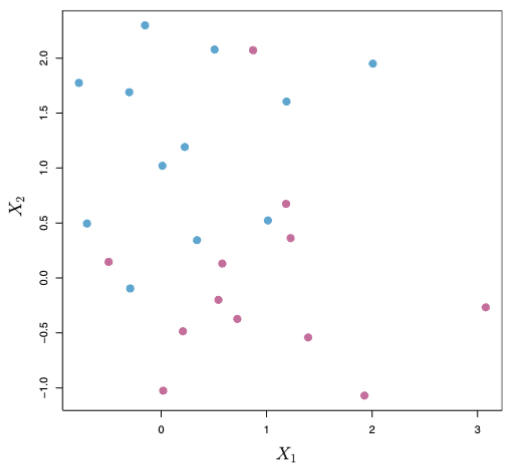
\includegraphics[width=0.5\textwidth]{fotos/55.png}
\caption{Un conjunto de datos en el que no existe un hiperplano separador.}
\label{fig:9.4}
\end{figure}


\subsection{Clasificador de vectores de soporte}

El problema de optimización que hay que resolver es cuadrático con restricciones de desigualdad lineales, y por lo tanto es un problema de optimización convexo. Recordemos que este problema era 
\begin{align}
\underset{\beta_0, \beta_1, \dots, \beta_p, \xi_1, \dots, \xi_n}{\text{minimize }} & M \\
\text{sujeto a } \quad & \sum_{j = 1}^p \beta_j^2 = 1 \\
&y_i (\beta_0 + \beta_1 x_{i1} + \beta_2 x_{i2} + \ldots + \beta_p x_{ip}) \geq M(1 - \xi_i) \\
&\xi_i \geq 0, \quad \sum_{i = 1}^n \xi_i \leq \text{constante}
\end{align}

\noindent y lo reformulamos como 
\begin{equation}
\min \|\beta\| \quad \text{sujeto a}
\begin{cases}
y_i (x_i^T \beta + \beta_0) \geq 1 - \xi_i \quad \forall i, \\
\xi_i \geq 0, \sum \xi_i \leq \text{constante}.
\end{cases}
\label{eq:12.7}
\end{equation}

\noindent No obstante, es computacionamente conveniente reescribirlo como 
\begin{align}
\underset{\beta, \beta_0}{\text{minimize }} & \frac{1}{2} ||\beta||^2 + C\sum_{i = 1}^N \xi_i \notag \\
\text{sujeto a } \quad & \xi_i \geq 0, \quad y_i(x_i^T \beta + \beta_0) \geq 1 - \xi_i \; \forall i \label{eq:12.8} \\
\end{align}

donde el parámetro de ``costo'' $C$ reemplaza la constante en (\ref{eq:12.7}); el caso separable corresponde a $C \to \infty$ (es decir, actúa como el inverso de los parámetros de regularización que hemos visto hasta ahora). La función de Lagrange (primal) es
\begin{equation}
L_P = \frac{1}{2} \|\beta\|^2 + C \sum_{i=1}^N \xi_i - \sum_{i=1}^N \alpha_i [y_i (x_i^T \beta + \beta_0) - (1 - \xi_i)] - \sum_{i=1}^N \mu_i \xi_i
\label{eq:12.9}
\end{equation}

que minimizamos con respecto a $\beta$, $\beta_0$ y $\xi_i$. Al igualar las respectivas derivadas a cero, obtenemos
\begin{align}
\beta &= \sum_{i=1}^N \alpha_i y_i x_i \label{eq:12.10} \\
0 &= \sum_{i=1}^N \alpha_i y_i \label{eq:12.11} \\
\alpha_i &= C - \mu_i, \quad \forall i \label{eq:12.12}
\end{align}

así como las restricciones de positividad $\alpha_i, \mu_i, \xi_i \geq 0 \quad \forall i$. Al sustituir (\ref{eq:12.10})–(\ref{eq:12.12}) en (\ref{eq:12.9}), obtenemos la función objetivo dual de Lagrange (Wolfe)
\begin{equation}
L_D = \sum_{i=1}^N \alpha_i - \frac{1}{2} \sum_{i=1}^N \sum_{i'}^N \alpha_i \alpha_{i'} y_i y_{i'} x_i^T x_{i'},
\label{eq:12.13}
\end{equation}

que da un límite inferior a la función objetivo (\ref{eq:12.8}) para cualquier punto factible. Maximizamos $L_D$ sujeto a $0 \leq \alpha_i \leq C$ y $\sum_{i=1}^N \alpha_i y_i = 0$. Además de (\ref{eq:12.10})–(\ref{eq:12.12}), las condiciones de Karush-Kuhn-Tucker incluyen las restricciones
\begin{align}
\alpha_i [y_i (x_i^T \beta + \beta_0) - (1 - \xi_i)] &= 0, \label{eq:12.14}\\
\mu_i \xi_i &= 0, \label{eq:12.15} \\
y_i (x_i^T \beta + \beta_0) - (1 - \xi_i) &\geq 0, \label{eq:12.16}
\end{align}

para $i = 1, \ldots, N$. Juntas, las ecuaciones (\ref{eq:12.10})–(\ref{eq:12.16}) caracterizan de manera única la solución al problema primal y dual. De (\ref{eq:12.10}) vemos que la solución de $\beta$ tiene la forma 
\begin{equation}
\hat{\beta} = \sum_{i=1}^N \hat{\alpha}_i y_i x_i
\label{eq:12.17}    
\end{equation}

con coeficientes $\hat{\alpha}_i > 0$ solo para aquellas observaciones $i$ para las cuales las restricciones en (\ref{eq:12.16}) se cumplen exactamente (debido a (\ref{eq:12.14})). Estas observaciones se llaman vectores de soporte, ya que $\hat{\beta}$ se representa solo en términos de ellas. Entre estos puntos de soporte, algunos se encontrarán en el borde del margen ($\hat{\xi}_i = 0$), y por lo tanto, de (\ref{eq:12.15}) y (\ref{eq:12.12}) se caracterizarán por $0 < \hat{\alpha}_i < C$; el resto ($\hat{\xi}_i > 0$) tienen $\hat{\alpha}_i = C$. De (\ref{eq:12.14}) podemos ver que cualquiera de estos puntos del margen ($0 < \hat{\alpha}_i, \hat{\xi}_i = 0$) puede usarse para resolver $\beta_0$, y típicamente usamos un promedio de todas las soluciones para la estabilidad numérica. Para calcular los $\xi$ de puntos que no están sobre el margen, se necesita conocer $\beta$ y $\beta_0$. Es necesario saber obtener los vectores de soporte a partir de $alpha_i$ y $C$. \\

Maximizar el dual (\ref{eq:12.13}) es un problema de programación cuadrática convexa más simple que el primal (\ref{eq:12.9}), y puede resolverse con técnicas estándar. Dadas las soluciones $\hat{\beta}_0$ y $\hat{\beta}$, la función de decisión puede escribirse como
\begin{equation}
    \hat{G}(x) = \text{sign}[\hat{f}(x)] = \text{sign}[x^T\hat{\beta} + \hat{\beta}_0].
\end{equation}

donde el signo dice la clase (positivo corresponde a +1 y negativo a -1) y la magnitud da la distancia al hiperplano. \\

\noindent El hiperparámetro de este proceso es $C$. En regresión Ridge, por ejemplo, con $\lambda = 0$ teníamos un modelos sobreaprendido (mínimos cuadrados), y con $\lambda$ muy grande teníamos un modelo subaprendido. En el caso de los clasificadores de vectores de soporte, un $C$ muy grande da un modelo sobreaprendido (que no permite $\xi$ con valores muy altos), por lo que habrá pocos vectores de soporte. Sin embargo, un $C$ muy pequeño nos da un modelo subaprendido, permite muchos $\xi$ con valores altos y, por tanto, habrá muchos vectores de soporte; esto es similar a lo que veíamos para KNN. Por tanto, $C$ actúa como el inverso de una constante de regularización. \\


\subsubsection{Frontera de decisión no lineal}

En el caso de que las clases no sean linealmente separables, con LDA podíamos recurrir a la siguiente transformación: se genera una transformación de los datos de entrada, añadiendo nuevas variables que sean combinaciones de estas o transformaciones de cada una. Esto expande el espacio de entrada, lo que no da un espacio multidimensional mayor sobre el que las clases sí son linealmente separables. Al aplicar LDA sobre este nuevo espacio, se obtiene una frontera de decisión lineal que, al proyectar sobre el espacio bidimensional, da la impresión de curva y se adapta a los datos. \\

Las máquinas de vectores de soporte harán algo similar a esto, pero sin dar a conocer que transformaciones se hacen sobre los datos.

\section{Máquinas de vectores de soporte}

El clasificador de vectores de soporte descrito hasta ahora encuentra límites lineales en el espacio de características de entrada. Al igual que con otros métodos lineales, podemos hacer el procedimiento más flexible ampliando el espacio de características utilizando expansiones de base como polinomios o splines. Generalmente, los límites lineales en el espacio ampliado logran una mejor separación de clases en el entrenamiento y se traducen en límites no lineales en el espacio original. Una vez que se seleccionan las funciones base $h_m(x)$, $m = 1, \ldots, M$, el procedimiento es el mismo que antes. Ajustamos el clasificador SV utilizando características de entrada $h(x_i) = (h_1(x_i), h_2(x_i), \ldots, h_M(x_i))$, $i = 1, \ldots, N$, y producimos la función (no lineal) $\hat{f}(x) = h(x)^T \hat{\beta} + \hat{\beta}_0$. El clasificador es $\hat{G}(x) = \text{sign}(\hat{f}(x))$ como antes. \\

El clasificador de máquinas de vectores de soporte es una extensión de esta idea, donde la dimensión del espacio ampliado puede llegar a ser muy grande, infinita en algunos casos. Podría parecer que los cálculos se volverían prohibitivos. También parecería que con suficientes funciones base, los datos serían separables y ocurriría sobreajuste. Primero mostramos cómo la tecnología SVM aborda estos problemas. Luego vemos que, de hecho, el clasificador SVM está resolviendo un problema de ajuste de funciones utilizando un criterio particular y una forma de regularización, y es parte de una clase mucho más grande de problemas que incluye los splines de suavizado. \\

Antes de ver cómo se hace esto, reformulemos el clasificador de vectores de soporte en función del producto interno de las observaciones:
\begin{equation}
\langle x_i, x_j \rangle = \sum_{j = 1}^p x_{ij} x_{i'j}
\end{equation}

\noindent Así, el problema anterior queda definido por 
\begin{align}
G(x) &= \text{sign} [x^T \beta + \beta_0] \\
\beta &= \sum_{i=1}^N \alpha_i y_i x_i \\
f(x) &= \beta_0 + \sum_{i = 1}^N \alpha_i y_i \langle x, x_i \rangle
\end{align}

\noindent donde recordemos que $x_i$ es un vector de $p$ componentes. Ahora, el problema de optimización anterior lo podemos escribir, en función del producto interno y usando ya las transformaciones $h(x_i)$ (que desconocemos) como
\begin{equation}
L_D = \sum_{i = 1}^N \alpha_i - \frac{1}{2} \sum_{i = 1}^N \sum_{i' = 1}^N \alpha_i \alpha_{i'} y_i y_{i'} \langle h(x_i), h(x_{i'}) \rangle
\end{equation}

\noindent y la solución la podemos escribir como 
\begin{equation}
f(x) = h(x)^T \beta + \beta_0 = \sum_{i = 1}^N \alpha_i y_i \langle h(x), h(x_i) \rangle + \beta_0
\end{equation}

Como vemos en la ecuación anterior, no se necesita conocer la transformación $h(\cdot)$ para representar el clasificador lineal $f(x)$ o calcular sus coeficientes, simplemente basta con conocer el producto interno en el espacio de características ampliado. Esto es lo que conocemos como la función \textit{kernel}:
\begin{equation}
K(x, x') = \langle h(x), h(x') \rangle
\end{equation}

donde $K$ debe ser una función simétrica semidefinida positiva. El \textit{kernel} nos permite entonces modelar el producto interno, y podemos entenderlo como una medida de la similaridad entre dos vectores. Si nos fijamos en la solución en función del \textit{kernel}, 
\begin{equation}
\hat{f}(x) = \sum_{i = 1}^N \hat{\alpha}_i y_i K(x, x_i) + \hat{\beta}_0
\end{equation}

\noindent siendo $\hat{\alpha}_i$ positivo y la etiqueta $y_i$ positiva o negativa. Si el ejemplo que queremos categorizar se parece mucho a un vector de soporte, el producto interno (\textit{kernel}) será grande y positivo, por lo que la categoría de ese vector de soporte contribuirá mucho a la categoría del vector. Si son perpendiculares, el producto interno será 0, y si es opuesto, será negativo. \\

La ventaja de trabajar con el \textit{kernel} es clara: computacionalmente más eficiente, ya que solo es ncesario calcular $n(n-1)/2$ productors internos, y no es necesario trabajar de forma explícita en el espacio transformado. Opciones comunes de \textit{kernel} son:
\begin{itemize}
\item \textit{Kernel lineal:} Este es el caso más simple, que se corresponde con los clasificadores de vectores de soporte (SVC):
\begin{equation}
K(x_i, x_{i'}) = \langle x, x' \rangle
\end{equation}
\item La combinación de un SVC con un \textit{kernel} no lineal nos da una SVM: 
\begin{itemize}
\item \textit{Kernel polinómico de grado $d$:} 
\begin{equation}
K(x_i, x_{i'}) = (1 + \langle x_i, x_{i'} \rangle)^d = \left(1 + \sum_{j = 1}^p x_{ij} x_{i'j}\right)^d
\end{equation}

A menor grado del polinomio, más riesgo de subaprendizaje. Este kernel es más simple que el radial, que veremos a continuación.
\item \textit{Kernel radial:}
\begin{equation}
K(x_i, x_{i'}) = \exp \left( - \gamma \sum_{j = 1}^p (x_{ij} - x_{i'j})^2 \right)
\end{equation}

Aquí, vemos que $\gamma$ representa el inverso de la varianza de una graussiana, y la resta da la diferencia entre lo que evaluamos y los vectores de soporte. Por tanto, con este \textit{kernel} estamos tomando el elemento a evaluar, $x$, como la media de una gaussiana de varianza $\gamma$. Cuanto más se aleje el vector de soporte de este valor medio $x$, menor será el valor del \textit{kernel}. La similaridad en este caso está acotada entre 0 y 1. \\

Ahora, veamos como influye aquí $\gamma$ en el aprendizaje. Con una gaussiana estrecha, habrá pocos vectores de soporte que contribuyen a la clasificación efectiva de ese ejemplo, por lo que se sobreajusta, como ocurría con KNN. Entonces, si $\sigma^2$ es pequeño, $\gamma$ es grande, llevando al extremo, solo contribuirá un único vector de soporte. Si por el contrario la gaussiana es grande ($\sigma^2$ grande), $\gamma$ será pequeño y habrá riesgo de subaprendizaje porque, llevado al extremo, todos los vectores de soporte contribuirán a la clasificación.
\end{itemize}
\end{itemize}

\begin{figure}[h]
\centering
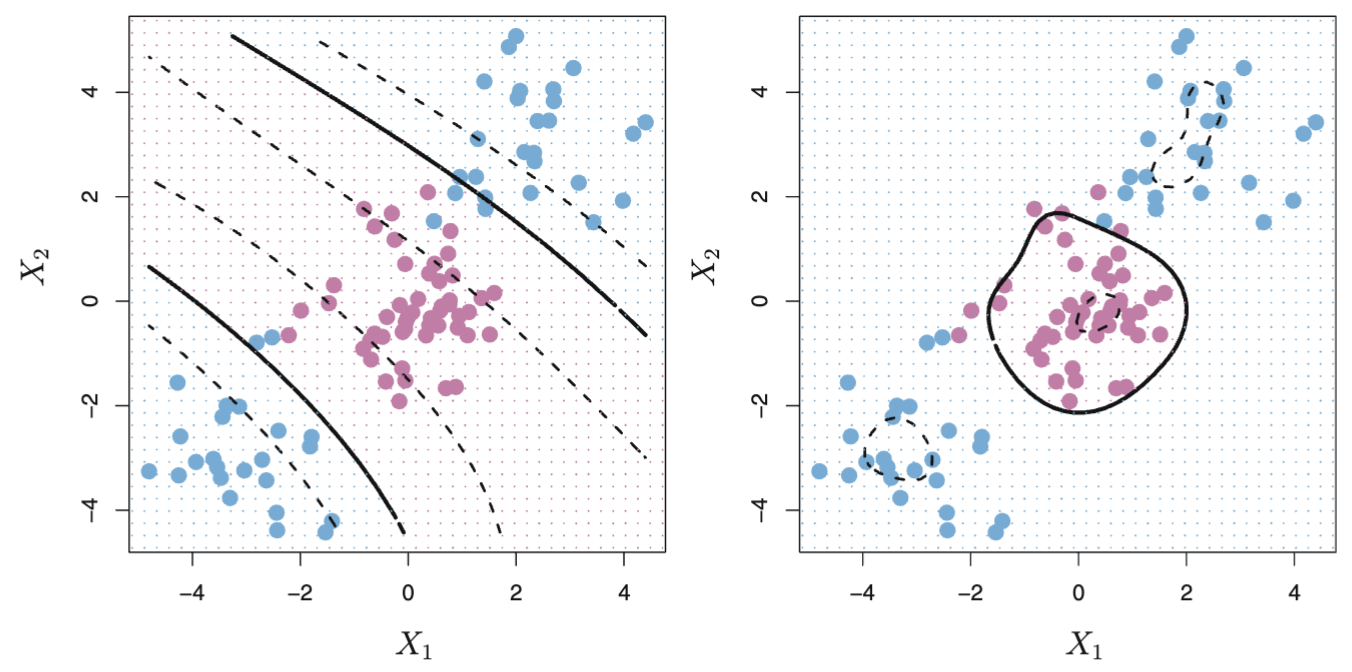
\includegraphics[width=0.5\textwidth]{fotos/57.png}
\caption{Ejemplo de \textit{kernel} polinómico (grado 3) y \textit{kernel} radial. En el kernel polinómico, los margenes son los huecos comprendidos entre las líneas discontinuas, donde se encuentran ambas líneas continuas; todos los puntos dentro de estos márgenes son vectores de soporte. Para el caso de la gaussiana es más complicado de ver: básicamente, los puntos que están dentro de los círculos discontinuos son los que están fuera del margen y no son vectores de soporte; el resto, son los vectores de soporte.}
\label{fig:12.2}
\end{figure}

\begin{example}
Usamos un conjunto de datos de enefermedades cardiacas para comparar 
Primero ajustamos LDA y el clasificador de vectores de soporte a los datos de entrenamiento.
Nota que el clasificador de vectores de soporte es equivalente a un SVM utilizando un núcleo polinomial de grado $d = 1$.
El panel de la izquierda de la Figura 9.10 muestra curvas ROC (descritas en la Sección 4.4.3) para las predicciones del conjunto de entrenamiento tanto para LDA como para el clasificador de vectores de soporte.
Ambos clasificadores calculan puntuaciones de la forma

\begin{equation}
\hat{f}(X) = \hat{\beta}_0 + \hat{\beta}_1 X_1 + \hat{\beta}_2 X_2 + \dots + \hat{\beta}_p X_p
\end{equation}

para cada observación.
Para cualquier umbral dado $t$, clasificamos las observaciones en las categorías de enfermedad cardíaca o sin enfermedad cardíaca dependiendo de si $\hat{f}(X) < t$ o $\hat{f}(X) \geq t$.
La curva ROC se obtiene formando estas predicciones y calculando las tasas de falsos positivos y verdaderos positivos para una gama de valores de $t$.
Un clasificador óptimo se acercará a la esquina superior izquierda del gráfico ROC.
En este caso, LDA y el clasificador de vectores de soporte ambos se desempeñan bien, aunque existe una sugerencia de que el clasificador de vectores de soporte puede ser ligeramente superior.
El panel de la derecha de la Figura 9.10 muestra curvas ROC para SVMs usando un núcleo radial, con varios valores de $\gamma$.
A medida que $\gamma$ aumenta y el ajuste se vuelve más no lineal, las curvas ROC mejoran.
Usar $\gamma = 10^{-1}$ parece dar una curva ROC casi perfecta.
Sin embargo, estas curvas representan tasas de error de entrenamiento, lo que puede ser engañoso en términos de desempeño en nuevos datos de prueba.
La Figura 9.11 muestra curvas ROC calculadas en las 90 observaciones de prueba.
Observamos algunas diferencias con respecto a las curvas ROC de entrenamiento.
En el panel de la izquierda de la Figura 9.11, el clasificador de vectores de soporte parece tener una pequeña ventaja sobre LDA (aunque estas diferencias no son estadísticamente significativas).
En el panel de la derecha, el SVM usando $\gamma = 10^{-1}$, que mostró los mejores resultados en los datos de entrenamiento, produce las peores estimaciones en los datos de prueba.
Esto nuevamente es evidencia de que aunque un método más flexible a menudo produce tasas de error de entrenamiento más bajas, esto no necesariamente conduce a un mejor desempeño en datos de prueba.
Los SVMs con $\gamma = 10^{-2}$ y $\gamma = 10^{-3}$ se desempeñan de manera comparable al clasificador de vectores de soporte, y los tres superan al SVM con $\gamma = 10^{-1}$.
\end{example}

\section{10/12}


HAsta ahora solo podemos hacer clasificacion binaria. 

En 1vs1 para deshacer empate miramos los valores.

para mas de dos calses no funcionan bien. Para hacerlo con mas de dos, aprendemos varios modelos, uno para cada par de categorias. 


No funciona tan bien en regresion por su propia definicion (usar hiperplano de separacion)


\begin{example}
alpha = 0 para los vectores que no son de soporte. El de alpha menor que 1 esta sobre el margen, mientras que el de alpha 1 es el unico que no esta e ne l magrne. Beta sera alpha por el vector correspondeinte para todos losq eu so nvectores de soorte. Usando la e (1) de sus diapositivas, con esos tres calculamos 3 beta 0 y obtenemos beta. Una vez tenemos estos, para el resto de vec de soporte podemos calcular las epsilon correspondientes. Para el que no esta en el margen, tiene la distancia del margen al hiperplano es 1 margen, y como el que no es vector de siporte esta sobre el hiperplano, su epsilon es 1 (1 margen). M es el inverso del modulo de beta. los de epsilon mayor a uno seran los incorrectamente clasificados.   \\


alpha son los multipl. de Lagrange

para calcular beta hacer la suma ponderada por los alphas de todos los vec de soporte. Para beta 0 usar los vec justo en el margen y luego dar la media. PAra los vec de sop que no estan en el margen calcular epsilon (que no es cero). Para ver los incorrectamente clasif son los de epsilon mayor que 1. Diapositiva 17. (4), (1)
\end{example}

con c infinito queremos que los epsilon se vayan a cero (un hiperplano donde no entren vectores de soporte casi). A veces no puede encontrar 